% \section*{Vsebina}
% \begin{frame}[allowframebreaks]
%     \tableofcontents
% \end{frame}

\section{Uvod}

\begin{frame}{Ciljni primer}
  \begin{itemize}
    \item Želimo poznati napetosti in pomike v okolici stika
  \end{itemize}
  \centering
  \vspace{6ex}
  \includegraphics[width=\textwidth]{resources/fwo_shema.pdf}
\end{frame}

\section{Teorija linearne elastičnosti}

\begin{frame}{Opis gibanja in aksiomi}
  \vspace{0.5ex}
  \centering
  \includegraphics[width=0.65\textwidth]{resources/movement.pdf}
  \vspace{0.5ex}
  \begin{block}{Aksioma o gibalni in vrtilni količini}
    \vspace*{-3.5ex}
  \begin{align*}
    \ddt{} \int_B \dot{\vx}\, dm &= \int_B \vec{f}\, dV + \int_{\partial B} \vec{t}\, dS
    \\
    \ddt{} \int_B \dot{\vx} \times \vx\, dm &= \int_B \vec{f} \times \vx\, dV +
    \int_{\partial B} \vec{t} \times \vx\, dS
  \end{align*}
    \vspace*{-2.5ex}
  \end{block}
\end{frame}

\begin{frame}{Osnovne enačbe}
  \begin{itemize}
    \item Gibanje: $\rho \ddot{\vec{u}} = \div \sigma + \vec{f}$ \\[3ex] \pause
    \item Deformacija: $\eps = \frac12\left( \grad \vec{u} + \grad\vec{u}^\T + \cancel{\grad \vec{u}
      \grad\vec{u}^\T} \right)$ \\[3ex] \pause
    \item Hookov zakon: $\sigma = C : \eps$ \ \ ali \ \ $\sigma = \lambda \tr(\eps) I + 2\mu \eps$
      \\[3ex]  \pause
    \item[$\Rightarrow$] sledi \mbox{ } \\[3ex]
  \end{itemize}

  \begin{block}{Navierova enačba}
    \vspace{-1ex}
    \[
      \rho \ddot{\vec{u}} =
      (\lambda + \mu) \nabla(\nabla\cdot \vec{u}) + \mu \nabla^2 \vec{u} + \vec{f}
    \]
  \end{block} \pause
  stacionarna enačba, robni pogoji? % predpišejo $\vec{u}$ ali $\vec{t}$
\end{frame}

\section{Numerična metoda}

\begin{frame}{Uvod}
  \begin{itemize}
    \item Rešujemo enačbo
      \begin{align*}
        \mathcal{L} u = f& \quad \text{ na } \quad \Omega, \\
        \mathcal{R} u = g& \quad \text{ na } \quad \partial\Omega.
      \end{align*}
    \item Brezmrežna metoda, v močni obliki. \vspace{1ex}
      \begin{center}
      
\includegraphics[width=0.65\textwidth]{resources/domain_theoretical.pdf}
      \end{center}
  \end{itemize}
\end{frame}

\begin{frame}{Aproksimacija linearnega parcialnega diferencialnega operatorja}
  \begin{itemize}
    \item Ideja: \hfill $(\L u)(x) \approx (\L \hat{u})(x), \quad \displaystyle \hat{u}(x) = \sum_{i=1}^m
      \alpha_i b_i(x)$ \hfill \mbox{ } \\[2ex]
    \item  Zahtevamo interpolacijo v sosednjih točkah
      \[ \hat{u}(x_i) = u(x_i), \quad \forall x_i \text{ sosed } x \] \pause
    \item[$\Rightarrow$] sledi
      \[
        \begin{bmatrix}
        b_1(x_1) & \ldots & b_m(x_1) \\
        \vdots & \ddots & \vdots \\
        b_1(x_n) & \ldots & b_m(x_n)
        \end{bmatrix}
        \begin{bmatrix}
        \alpha_1 \\ \vdots \\ \alpha_m
        \end{bmatrix}
        =
        \begin{bmatrix}
        u_1 \\ \vdots \\ u_n
        \end{bmatrix}
      \]
  \end{itemize}
\end{frame}
\begin{frame}{Aproksimacija linearnega parcialnega diferencialnega operatorja}
  \begin{itemize}
    \item Sistem $B\alpha = u$ \\[2ex]
    \item Rešitev $\alpha =  (WB)^+W u$\\[2ex] \pause
    \item[$\Rightarrow$] sledi
    \[
      \hat{u}(x) = b(x)^\T\alpha = b(x)^\T(WB)^+W u
    \]  \pause \vspace{-2ex}
    \item[$\Rightarrow$] sledi
      \[ (\L u)(x) \approx (\L \hat{u})(x) = \underbrace{(\L b)(x)^\T (WB)^+W}_{\varphi(x)} u \]
  \end{itemize}
\end{frame}

\begin{frame}{Numerično reševanje}
  \begin{enumerate}
    \item Izračunamo $\varphi(x)$ za vsak $x$ in nastavimo enačbe \[ \varphi(x)u = f \] \\[4ex]
    \item Zložimo v matriko $A$ in nastavimo robne pogoje\\[10ex]
    \item Rešimo razpršen sistem $Au = f$
  \end{enumerate}
\end{frame}

\begin{frame}{Implementacija}
  \centering
  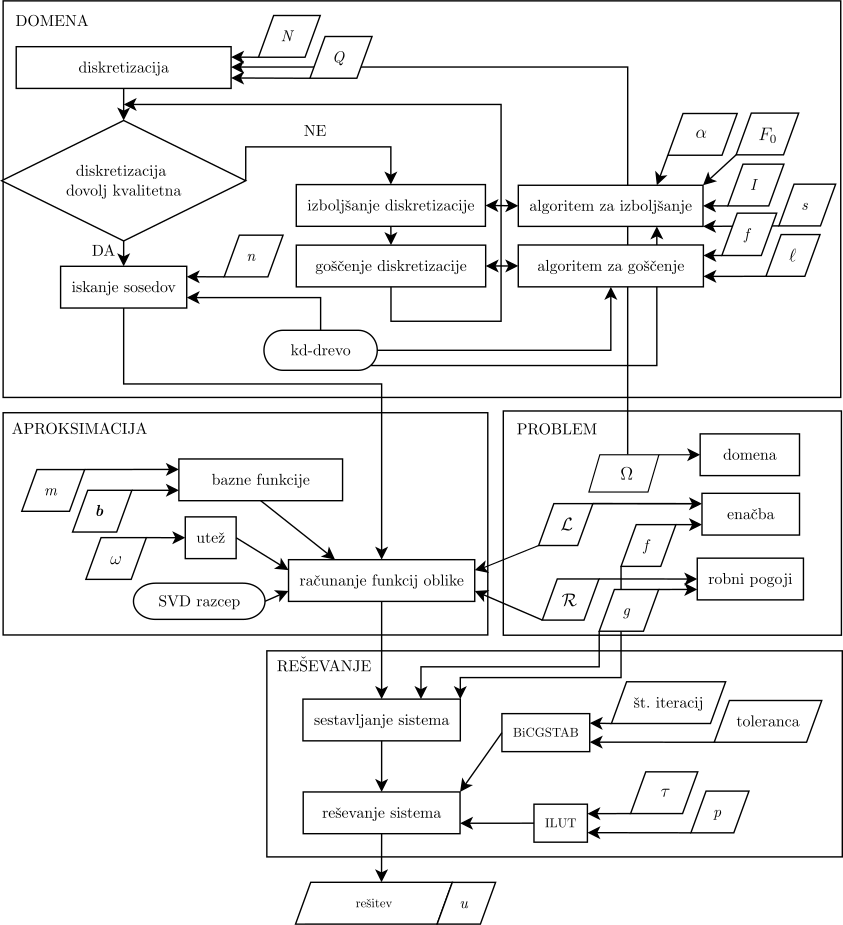
\includegraphics[height=0.9\textheight]{resources/diagram_finished.pdf}
\end{frame}

\section{Analize in zgledi}

\begin{frame}{Primerjava s FDM}
  \vspace{3ex}
  \includegraphics[width=\textwidth]{resources/lap1d_convergence.pdf}
\end{frame}

\begin{frame}{Difuzijska enačba}
  \vspace{1ex}
  \includegraphics[height=0.4\textheight]{resources/miki.png}
  \hspace{-10pt}
  \includegraphics[height=0.4\textheight]{resources/poisson_weird1.png}
  \hspace{0pt}
  \includegraphics[height=0.4\textheight]{resources/poisson_weird2.png}

  \vspace{1ex}

  \mbox{ }
  \hfill
  \includegraphics[height=0.4\textheight]{resources/neu.png}
  \hspace{10pt}
  \includegraphics[height=0.4\textheight]{resources/poisson_weird3.png}
  \hfill
  \mbox{ }
\end{frame}

% \begin{frame}{Vpet nosilec -- matrika}
%   \centering
%   \vspace{2ex}
%   \includegraphics[height=0.8\textheight]{resources/cantilever_beam_matrix_example.pdf}
% \end{frame}

% \begin{frame}{Vpet nosilec}
%   \centering
%   \includegraphics[width=\textwidth]{resources/cantilever_beam_convergence.pdf}
% \end{frame}

\begin{frame}{Vpet nosilec -- rešitev}
  \centering
  \vspace{3ex}
  \includegraphics[width=\textwidth]{resources/cantilever_beam_with_holes.png}
\end{frame}

\begin{frame}{Hertzev kontakt -- domena}
  \centering
  \vspace{3ex}
  \includegraphics[width=\textwidth]{resources/hertzian_refined_domain.png}
\end{frame}

\begin{frame}{Hertzev kontakt -- konvergenca}
  \centering
  \vspace{3ex}
  \includegraphics[width=\textwidth]{resources/hertzian_refine_levels_convergence.pdf}
\end{frame}

\begin{frame}{Hertzev kontakt -- rešitev}
  \centering
  \vspace{3.5ex}
  \includegraphics[width=\textwidth]{resources/hertzian_solution_deformed_vm.png}
\end{frame}

\begin{frame}{Ciljni primer}
  \centering
  \vfill
  \includegraphics[width=\textwidth]{resources/fwo_shema.pdf}
  \vfill
\end{frame}

\begin{frame}{Ciljni primer -- rešitev}
  \centering
  \vfill
  \includegraphics[width=\textwidth]{resources/fwo_solution.png}
  \vfill
\end{frame}

\section{Zaključek}
\begin{frame}
  \vfill
  \begin{block}{Nauk}
    Z brezmrežnimi metodami je mogoče uspešno in učinkovito reševati probleme iz linearne
    elastomehanike.
  \end{block}

  \vfill
  Hvala za pozornost!
\end{frame}
